%%%%%%%%%%%%%%%%%%%%%%%%%%%%%%%%%%%%%%%%%
% Lachaise Assignment
% LaTeX Template
% Version 1.0 (26/6/2018)
%
% This template originates from:
% http://www.LaTeXTemplates.com
%
% Authors:
% Marion Lachaise & François Févotte
% Vel (vel@LaTeXTemplates.com)
%
% License:
% CC BY-NC-SA 3.0 (http://creativecommons.org/licenses/by-nc-sa/3.0/)
%
%%%%%%%%%%%%%%%%%%%%%%%%%%%%%%%%%%%%%%%%%

%---------------------------------------------------------------------------------
%	PACKAGES AND OTHER DOCUMENT CONFIGURATIONS
%---------------------------------------------------------------------------------

\documentclass{article}

%%%%%%%%%%%%%%%%%%%%%%%%%%%%%%%%%%%%%%%%%
% Lachaise Assignment
% Structure Specification File
% Version 1.0 (26/6/2018)
%
% This template originates from:
% http://www.LaTeXTemplates.com
%
% Authors:
% Marion Lachaise & François Févotte
% Vel (vel@LaTeXTemplates.com)
%
% License:
% CC BY-NC-SA 3.0 (http://creativecommons.org/licenses/by-nc-sa/3.0/)
%
%%%%%%%%%%%%%%%%%%%%%%%%%%%%%%%%%%%%%%%%%

%----------------------------------------------------------------------------------------
%	PACKAGES AND OTHER DOCUMENT CONFIGURATIONS
%----------------------------------------------------------------------------------------

\usepackage{amsmath,amsfonts,stmaryrd,amssymb,mathtools} % Math packages

\usepackage{enumerate} % Custom item numbers for enumerations

\usepackage[ruled]{algorithm2e} % Algorithms

\usepackage[framemethod=tikz]{mdframed} % Allows defining custom boxed/framed environments

\usepackage{listings} % File listings, with syntax highlighting
\lstset{
	basicstyle=\ttfamily, % Typeset listings in monospace font
}

%----------------------------------------------------------------------------------------
%	DOCUMENT MARGINS
%----------------------------------------------------------------------------------------

\usepackage{geometry} % Required for adjusting page dimensions and margins

\geometry{
	paper=a4paper, % Paper size, change to letterpaper for US letter size
	top=2.5cm, % Top margin
	bottom=3cm, % Bottom margin
	left=2.5cm, % Left margin
	right=2.5cm, % Right margin
	headheight=14pt, % Header height
	footskip=1.5cm, % Space from the bottom margin to the baseline of the footer
	headsep=1.2cm, % Space from the top margin to the baseline of the header
	%showframe, % Uncomment to show how the type block is set on the page
}

%----------------------------------------------------------------------------------------
%	FONTS
%----------------------------------------------------------------------------------------

\usepackage[utf8]{inputenc} % Required for inputting international characters
\usepackage[T1]{fontenc} % Output font encoding for international characters

\usepackage{XCharter} % Use the XCharter fonts

%----------------------------------------------------------------------------------------
%	COMMAND LINE ENVIRONMENT
%----------------------------------------------------------------------------------------

% Usage:
% \begin{commandline}
%	\begin{verbatim}
%		$ ls
%
%		Applications	Desktop	...
%	\end{verbatim}
% \end{commandline}

\mdfdefinestyle{commandline}{
	leftmargin=10pt,
	rightmargin=10pt,
	innerleftmargin=15pt,
	middlelinecolor=black!50!white,
	middlelinewidth=2pt,
	frametitlerule=false,
	backgroundcolor=black!5!white,
	frametitle={Command Line},
	frametitlefont={\normalfont\sffamily\color{white}\hspace{-1em}},
	frametitlebackgroundcolor=black!50!white,
	nobreak,
}

% Define a custom environment for command-line snapshots
\newenvironment{commandline}{
	\medskip
	\begin{mdframed}[style=commandline]
}{
	\end{mdframed}
	\medskip
}

%----------------------------------------------------------------------------------------
%	FILE CONTENTS ENVIRONMENT
%----------------------------------------------------------------------------------------

% Usage:
% \begin{file}[optional filename, defaults to "File"]
%	File contents, for example, with a listings environment
% \end{file}

\mdfdefinestyle{file}{
	innertopmargin=1.6\baselineskip,
	innerbottommargin=0.8\baselineskip,
	topline=false, bottomline=false,
	leftline=false, rightline=false,
	leftmargin=2cm,
	rightmargin=2cm,
	singleextra={%
		\draw[fill=black!10!white](P)++(0,-1.2em)rectangle(P-|O);
		\node[anchor=north west]
		at(P-|O){\ttfamily\mdfilename};
		%
		\def\l{3em}
		\draw(O-|P)++(-\l,0)--++(\l,\l)--(P)--(P-|O)--(O)--cycle;
		\draw(O-|P)++(-\l,0)--++(0,\l)--++(\l,0);
	},
	nobreak,
}

% Define a custom environment for file contents
\newenvironment{file}[1][File]{ % Set the default filename to "File"
	\medskip
	\newcommand{\mdfilename}{#1}
	\begin{mdframed}[style=file]
}{
	\end{mdframed}
	\medskip
}

%----------------------------------------------------------------------------------------
%	NUMBERED QUESTIONS ENVIRONMENT
%----------------------------------------------------------------------------------------

% Usage:
% \begin{question}[optional title]
%	Question contents
% \end{question}

\mdfdefinestyle{question}{
	innertopmargin=1.2\baselineskip,
	innerbottommargin=0.8\baselineskip,
	roundcorner=5pt,
	nobreak,
	singleextra={%
		\draw(P-|O)node[xshift=1em,anchor=west,fill=white,draw,rounded corners=5pt]{%
		Question\questionTitle};
	},
}

\newcounter{Question} % Stores the current question number that gets iterated with each new question

% Define a custom environment for numbered questions
\newenvironment{question}[1][\unskip]{
	\bigskip
	\stepcounter{Question}
	\newcommand{\questionTitle}{~#1}
	\begin{mdframed}[style=question]
}{
	\end{mdframed}
	\medskip
}

%----------------------------------------------------------------------------------------
%	WARNING TEXT ENVIRONMENT
%----------------------------------------------------------------------------------------

% Usage:
% \begin{warn}[optional title, defaults to "Warning:"]
%	Contents
% \end{warn}

\mdfdefinestyle{warning}{
	topline=false, bottomline=false,
	leftline=false, rightline=false,
	nobreak,
	singleextra={%
		\draw(P-|O)++(-0.5em,0)node(tmp1){};
		\draw(P-|O)++(0.5em,0)node(tmp2){};
		\fill[black,rotate around={45:(P-|O)}](tmp1)rectangle(tmp2);
		\node at(P-|O){\color{white}\scriptsize\bf !};
		\draw[very thick](P-|O)++(0,-1em)--(O);%--(O-|P);
	}
}

% Define a custom environment for warning text
\newenvironment{warn}[1][Warning:]{ % Set the default warning to "Warning:"
	\medskip
	\begin{mdframed}[style=warning]
		\noindent{\textbf{#1}}
}{
	\end{mdframed}
}

%----------------------------------------------------------------------------------------
%	INFORMATION ENVIRONMENT
%----------------------------------------------------------------------------------------

% Usage:
% \begin{info}[optional title, defaults to "Info:"]
% 	contents
% 	\end{info}

\mdfdefinestyle{info}{%
	topline=false, bottomline=false,
	leftline=false, rightline=false,
	nobreak,
	singleextra={%
		\fill[black](P-|O)circle[radius=0.4em];
		\node at(P-|O){\color{white}\scriptsize\bf i};
		\draw[very thick](P-|O)++(0,-0.8em)--(O);%--(O-|P);
	}
}

% Define a custom environment for information
\newenvironment{info}[1][Info:]{ % Set the default title to "Info:"
	\medskip
	\begin{mdframed}[style=info]
		\noindent{\textbf{#1}}
}{
	\end{mdframed}
}
 % Include the file specifying the document structure and custom commands
\usepackage{minted}
\usepackage{tikz}
\usepackage{listofitems} % for \readlist to create arrays
\tikzstyle{mynode}=[thick,draw=blue,fill=blue!20,circle,minimum size=22]
\usepackage{fancyvrb}
\usepackage{amsmath}
%\usemintedstyle{gruvbox-light}
\usepackage{tabularx}
\usepackage{verbatim}
\usepackage{listings}
\usepackage{booktabs}
\usepackage{float}
\usepackage{graphicx}
\usepackage{subcaption}
\graphicspath{{./figs/}}
\usepackage{amsfonts,stmaryrd,amssymb,mathtools,hyperref,centernot} % Math packages
\hypersetup{
    colorlinks=true,
    linkcolor=blue,
    filecolor=magenta,
    urlcolor=cyan,
}
%---------------------------------------------------------------------------------
%	ASSIGNMENT INFORMATION
%---------------------------------------------------------------------------------

\title{An Investigation of the Response of a Three-Layer Neural Network to Randomized SVD and Truncated SVD} % Title of the assignment

\author{Benjamin Keene --- \texttt{benkeene@knights.ucf.edu}} % Author name and email address

\date{University of Central Florida --- \today} % University, school and/or department name(s) and a date

%---------------------------------------------------------------------------------

\begin{document}

\maketitle % Print the title

{
	\hypersetup{linkcolor=black}
	\tableofcontents
}

\section{Introduction}
In this project we test the performance of a neural network's ability to classify handwritten digits from MNIST.
We will present the layout of the network, present its baseline performance without modifications.
Then, we will show the ability of the network to withstand compression of its weights via SVD while maintaining relatively accurate classification.

\subsection{Implementation and network design}
Our neural network takes $28 \times 28$ resolution images from MNIST and returns a value from $\{0,1,...,9\}$ as classification.
The layers of the network have the following structure:

\inputminted{python}{snippets/struct.py}

The number and size of the hidden layers is restricted by the platform we are training on.

\bigskip

Important to state, all layers (except for the final layer) have greater than 10 neurons.
If any layer had at most 10 neurons, then after compression we're likely to lose ability in classification of the 10 distinct digits of MNIST.

That is, applying a dimension reduction filter which reduces the rank of a weight matrix below 10 seems counterproductive to classification.

\bigskip

For our optimizer, we use stochastic gradient descent with a learning rate $lr = 10^{-2}$.

\subsection{Hardware}

This network was trained on the following platform:
\begin{itemize}
	\item OS: Windows 11 Pro
	\item CPU: Intel i7-12700k
	\item RAM: 48GB
	\item GPU: NVIDIA GTX 1080
	\item SSD: Samsung 980 NVMe
\end{itemize}

While capable, larger networks (combined with the SVD tensor operations) proved too cumbersome to reasonably analyze.

\subsection{Randomized SVD}

The paper \emph{Finding Structure with Randomness: Probabilistic Algorithms for Constructing Approximate Matrix Decompositions} by Halko, Martinsson, Tropp. (2010, December) demonstrates a novel method for constructing low-rank approximations.

\bigskip

While not the focus of this project, the algorithm for the randomized SVD is given.
\begin{center}
	\begin{minipage}{0.5\linewidth} % Adjust the minipage width to accomodate for the length of algorithm lines
		\begin{algorithm}[H]
			\KwIn{$A \in \mathbb{R}^{m \times n}$\\Target rank: $k$\\Oversampling parameter: $p$}  % Algorithm inputs
			\KwResult{$U$, $\Sigma$, $V^T$ in an SVD of $QQ^TA$} % Algorithm outputs/results
			\medskip
			Stage \textbf{A}
			\begin{enumerate}
				\item Draw $k+p$ random normal vectors $\omega_i$ in $\mathbb{R}^n$, forming $\Omega$
				\item Form the product $Y = A \Omega$
				\item Calculate the $m \times (k + p)$ matrix $Q$ from the $QR$ factorization of $Y$
			\end{enumerate}
			Stage \textbf{B}
			\begin{enumerate}
				\item Calculate an SVD of $Q^TA = \tilde{U} \Sigma V^T$.
				\item Left multiply this SVD by $Q$, where $Q\tilde{U} : = U$
			\end{enumerate}
			
			{\bf return} $U, \Sigma, V^T$ such that $A \approx U \Sigma V^T$.
			\caption{\texttt{Randomized SVD}} % Algorithm name
		\end{algorithm}
	\end{minipage}
\end{center}

Loosely, the randomized SVD first calculates the matrix $Q$ with orthonormal columns whose range approximates that of $A$.
Finding such a $Q$ such that, given $A\in\mathbb{R}^{m \times n}$ and precision tolerance $\epsilon$,
\[\| A - QQ^TA\| \leq \epsilon\]
is called the \textit{fixed-precision approximation problem}.

\bigskip

Constructing this matrix $Q$ with $k + p$ orthonormal columns that satisfy

\[\| A - QQ^T A\| \approx \min_{\text{rank}(X) \leq k} \| A - X \|\]

is called the \textit{fixed-rank approximation problem}.
\bigskip

It turns out, that with few requirements on the hyperparamter $p$ (an oversampling parameter), we have very good bounds on the error above.
In expectation, this error
\[\mathbb{E} \| A - QQ^TA\| \leq \left[ 1 + \frac{4\sqrt{k+p}}{p-1} \cdot \sqrt{\min\{m,n\}} \right] \sigma_{k+1}\]
is at worst a polynomial factor of the next singular value of $A$.
Halko et al. present that with relatively small $p$, the probability that the above inequality fails is roughly proportional to $p^{-(k+1)}$.
While out of scope of this review, we can rest assured that the randomized SVD algorithm behaves well for our purposes.

\subsection{Truncated SVD}

For fun, we implement the "truncated SVD", the first $k$ rank-one matrices in the SVD corresponding to the $k$-dominant singular values $\sigma_1, \sigma_2, \ldots, \sigma_k$.

\bigskip

By Eckart-Young theorem, we have that this is the \textbf{best} rank $k$ approximation of $A$.

\begin{center}
	\begin{minipage}{0.5\linewidth} % Adjust the minipage width to accomodate for the length of algorithm lines
		\begin{algorithm}[H]
			\KwIn{$A \in \mathbb{R}^{m \times n}$\\Target rank: $k$}  % Algorithm inputs
			\KwResult{$A_k = \sum_{i=1}^k \sigma_i u_i v_i^T$} % Algorithm outputs/results
			\medskip
			\begin{enumerate}
				\item Calculate the SVD $A = U \Sigma V^T$
				\item Set $[\Sigma]_{ii} = 0$ for $i > k$
				\item Set $A_k = U \Sigma V^T$
			\end{enumerate}
			
			{\bf return} $A_k$
			\caption{\texttt{Truncated SVD}} % Algorithm name
		\end{algorithm}
	\end{minipage}
\end{center}



\newpage
\section{Performance Analysis}

Presented below is the percent error, loss, and runtime of each implementation.
The following parameters for randomized SVD and truncated SVD were used.
\begin{enumerate}
	\item Stock: No manipulation of weight matrices during training
	\item rSVD: After each epoch, approximate each weight matrix by a rank 10 approximation
	\item truncSVD: After each epoch, approximate the each weight matrix by the first 10 terms of its singular value decomposition
\end{enumerate}
\begin{figure}[!htbp]
	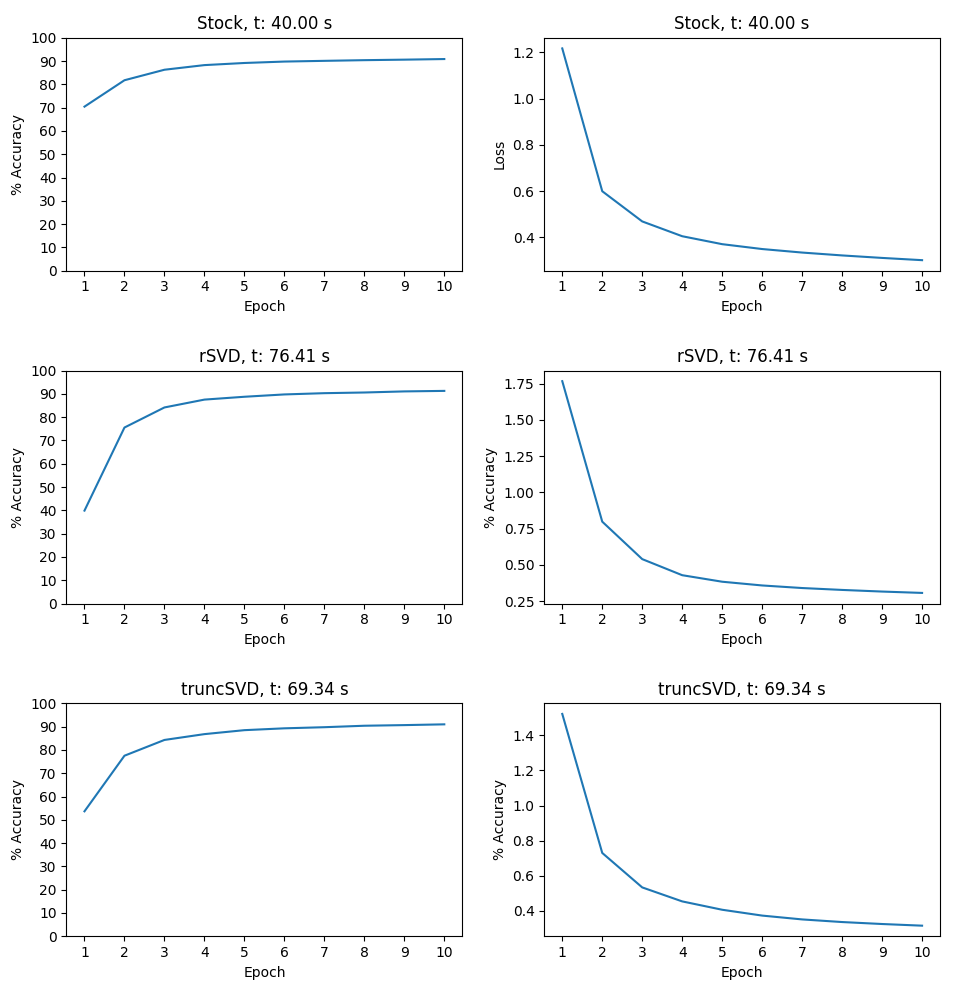
\includegraphics[scale=0.7]{Figure_1.png}
	\centering
	% Table generated by Excel2LaTeX from sheet 'Recurrence'
	\centering
	
	\label{tab:addlabel}%
\end{figure}%

Notice that each implementation (stock, rSVD, and truncSVD) reasonably learn to classify the digits.
The runtime however, is very poor in the rSVD and truncSVD implementations.

\section{Manipulating tensors in CUDA memory}
Shown below are the functions used to modify the tensors while preserving the gradient.
This was done via saving the model's state dictionary, manipulating the tensors directly, and reloading the altered weight matrices as the weights of a new model.
\inputminted{python}{snippets/rSVD.py}
\inputminted{python}{snippets/truncSVD.py}

\section{Remarks on how this might be useful}
We have shown how to implement Halko et al.'s randomized SVD as a compression algorithm against the weight matrices of a neural network, manipulating them in CUDA memory.
While we gain no extra accuracy by doing so, perhaps this is a feasible method for revealing the optimal rank (and further, the dimension) of a neural network's matrices.
Presented below is a possible heuristic:
\begin{center}
	\begin{minipage}{0.5\linewidth} % Adjust the minipage width to accomodate for the length of algorithm lines
		\begin{algorithm}[H]
			\KwIn{Weight matrices $A_1, A_2, ..., A_n$, tolerances $\epsilon_1, \epsilon_2, ..., \epsilon_n$}  % Algorithm inputs
			\KwResult{$k_1, k_2, ..., k_n$, the optimal rank of a low rank approximation of each matrix} % Algorithm outputs/results
			\medskip
			\begin{enumerate}
				\item For each $A_i \in \mathbb{R}^{m \times n}$ and $j \in \min\{m,n\}$:
				\subitem Calculate the loss, $\ell_{ij}$, of the network with $A_i$ approximated by its rank $j$ approximation via rSVD or truncSVD
				\subitem If $\ell_{ij} - \ell_{i(j+1)} \geq \epsilon_i$, then assign $A_i$ its rank $j$ approximation via rSVD or truncSVD
			\end{enumerate}
			
			{\bf return} $A_1, A_2, ..., A_n$
			\caption{\texttt{NN Rank Revealer}} % Algorithm name
		\end{algorithm}
	\end{minipage}
\end{center}

This algorithm is clearly unfeasible for large $n$, but interesting to think about.

\section{Conclusion}

To conclude, we've demonstrated how to manipulate the weight matrices of a neural network while training.
For the classification between 10 labels, the network behaves well when its matrices are replaced by rank 10 approximations via randomized SVD and truncated SVD.

\end{document}
